\chapter{Literature Review}\label{ch:litreview}
\section{Computer architectures}
With the exception of Babbage's Analytical Engine, probably the earliest
computer architecture to be formally described is that of the EDVAC (Electronic
Discrete Variable Automatic Computer), in 1945 by John von~Neumann in his
incomplete `First Draft of a Report on the EDVAC'. In it, von~Neumann describes
a fully programmable computer which is subdivided into six separate parts ---
Central Arithmetic (CA); Central Control (CC); Memory; Input; Output and
External Memory (at the time, this was intended to be something like punched
tape). These components were described using the human nervous sytem as an
analogy, with the CA, CC \& Memory acting as associative (linking) neurons, the
Input \& Output acting as sensory \& motor neurons respectively.
Von~Neumann also wanted to keep the computer as simple as possible, so suggested
that arithmetic operations (such as add and multiply) should not be overlapped,
and performed only one digit (this being before bits and bytes were named as
such) at a time. He also noted that external input/output should first be placed
into memory, rather than directly in/out of the CC or CA\@. This approach to
laying out the components of a computer stuck, and the approximate idea is still
used in modern processors today.\cite{FirstDraft}

\subsection{Register machines}
In the 1950s, logic gates and switches were largely implemented using the quite
large vacuum tubes and discrete transistors. With technology improving,
integrated circuits were invented, constructing logic components using layers of
metal and oxides on polished silicon. Initially, these were only used to
implement individual logic components for computers, replacing the diodes and
resistors used before, until in 1971, Intel released the 4004 microprocessor
(pictured in Figure~\ref{fig:4004}).
It was the first commercially available fully self contained microprocessor,
with its circuitry fabricated using the new `silicon gate' technology which is
why it was able to be designed and fabricated as one chip. It's worth noting
that Intel as a company didn't have much faith in this product, opting to
instead focus on its line of memory chips and partnering with a Japanese
electronic calculator firm, Busicom, to help finance the project. Nonetheless,
the 4004 was a huge commercial success with 4004 being produced for 10 solid
years and taking Intel to the giant in the computing world that it is
today.\cite{Aspray1997Intel}

\begin{figure}
  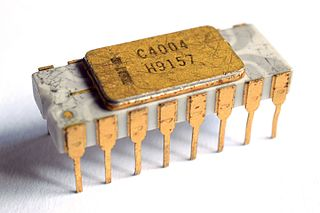
\includegraphics[width=0.5\textwidth]{imgs/Intel_C4004}
  \caption{Intel's 4004 microprocessor}\label{fig:4004}
\end{figure}

Very simply, register architectures work by having several named locations
(sometimes called the register file) within the CPU providing the fastest way to
access data in a system, often in a single CPU cycle, and are used to store and
retrieve intermediate results of computations. There are a number of different
types of register, with data registers storing numerical values, address
registers storing memory addresses for accessing system memory, general purpose
registers store both data and addresses, flag registers for storing truthiness
states of previous boolean test operations, and various others. There's also
often an instruction register that isn't accessible to the program running on
the CPU, but the CPU uses to refer to the current instruction being executed.
\cite{Mittal2016RegisterFile}\cite{Patterson2011Computer}

In register-based computing, there are two different competing architecture
types, Reduced Instruction Set Computers (RISC) and CISC (Complex Instruction
Set Computers). The RISC design uses the idea that a simple instruction set
enables a simpler microprocessor design, which can then run more instructions
per instruction cycle as a result. There's no formal definition of what
consitutes a RISC processor, but the general trend is that they have a single
instruction per type of operation, e.g.\ only having \texttt{load} and
\texttt{store} for memory accesses, rather than another instruction being able
to load or store to memory. Examples of RISC architectures include ARM, PowerPC
\& SPARC.\@ In recent years, the most powerful supercomputers have also taken to
using RISC processors, such as the `K Computer' which makes use of a processor
from the SPARC family.\cite{Yokokawa2011KCJ}

CISC designed processors are opposite in this regard, providing instructions
that can execute many operations within its execution cycle, sometimes taking
several cycles of the CPU to complete. For example, an \texttt{add} instruction
may be able to read from memory, perform the addition, and write back to memory
all by itself. There are often several instructions provided that implement the
same operation, but take different types of operands (e.g.\ registers, constants
or memory addresses). Examples of CISC architectures include IBM's System/360
and related mainframe architectures, the Z80 and the now ubiquitous x86 series
of processors.\cite{Patterson1980CRI}

\subsection{Stack machines}
The use of stacks as part of computation has been around almost as long as
computing itself, with Zuse's Z4 making use of them for subroutines in
1945,\cite{Speiser2000KZZ} and the Burroughs B5000 and its later models were
widely used in the 1960s as well.\cite{Organick2014Computer} At the time, stack
machines were considered to be the fastest computer architecture with the simple
instruction sets afforded by the stack greatly simplifying compiler design.
However, by the 1970s it had fallen out of favour, with improvements in compiler
design making memory-to-memory architectures (or register based) more
appealing. A common criticism was that stack architectures necessitated the use
of memory locations as imitations of registers, which slow the architectures
down.\cite{Myers1977CAS}

Instead of having named registers to store values as part of computations, stack
machines use a stack data structure to store the computationally active
variables. A stack is a so-called ``last in, first out'' (LI-FO) data structure,
meaning that the data that was last put into the structure is the first to be
pulled out again, usually with push \& pop operations, which place data onto the
stack and take it off again, respectively. This is compared to a data structure
such as a queue, which is a ``first in, first out'' structure. Stack machines
generally still have a couple of registers, although not often anything much
more than a program counter (for storing current position in the program) and a
flags register (for storing state about the last instruction for branching).

In the present day the use of stacks in computer architectures and instruction
sets is nearly exclusively limited to stack frames, to give the ability to do
context ``saving'' and ``loading'' with function calls, in favour of register
based computation. However, there is a notable exception --- the Java Virtual
Machine (JVM) uses a stack-based bytecode as its underlying assembly language
and virtual machine design.\cite{Schoeberl2005Design}

\section{Stack optimisations}

Because of the popularity of register architectures, higher level languages tend
to get designed with them particularly in mind. This means that the majority of
optimisation research for these languages gets done only for register
architectures. This is turn makes stack architectures less appealing in somewhat
of a spiral, making stack machines less and less appealing for additional usage.

Despite this, there has been significant work in the area of compiling these
`conventional' languages to a stack executation model. One of the main areas of
research has been focused on fixing the repeated loading and storing to the same
memory location that na{\"\i}ve compilation tends to produce.

Peephole optimisations are a method that can be applied to register and stack
architectures alike, with the effect of removing redundant instructions from
compiled code. McKeeman gives this name to this optimisation technique as it
involves looking at small sections of the generated object code, identifying
inefficient instruction segments and modifying them accordingly to generate
more efficient or shorter code. McKeeman uses ALGOL to give an example where an
assignment is followed by an addition.

\begin{minipage}{.25\textwidth}
  \centering
  \begin{lstlisting}[language=Algol]
X := Y;
Z := X + Z;
  \end{lstlisting}
\end{minipage}%
\begin{minipage}{.55\textwidth}
  Compiled code:
  \begin{lstlisting}
LDA Y ; load the accumulator from Y
STA X ; store the accumulator in X
LDA X ; load the accumulator from X
ADD Z ; add the contents of Z
STA Z ; store the accumulator in Z
  \end{lstlisting}
\end{minipage}

As long as the the store (\lstinline{STA X}) operation is nondestructive, the
subsequent \lstinline{LDA X} is unnecessary and can be removed. Peephole
optimisations such as this one generally make assumptions about which
instructions are expensive and should be replaced if possible. For example, for
stack machines a \lstinline{DUP} on the stack is generally much faster than a
\lstinline{LOAD} from memory. Another common peephole optimisation is `constant
collapsing'', where the compiler can compute the result of an arithmetic
operation between two or more constants, saving time calculating it at runtime.
However, peephole optimisers have to be careful not to optimise away behaviour
that can be reached elsewhere, for example with a label statement, which other
code elsewhere may be relying on.\cite{McKeeman1965Peephole}

One major area of interest of stack optimisations is the concept of stack
scheduling. That is, separating the code into blocks and optimising them by
removing extra memory accesses so that they can be executed concurrently. Baker
applies the concept to realtime systems, which have deadlines with which they
have to have completed their computation by, which has potentially disastrous
results if they do not.\cite{Baker1991Stack}

Koopman describes a method of optimisation of (generated) stack code that is
able to remove 91\% to 100\% of redundant local variable accesses. This is
achieved in 4 optimisation steps, in addition to the input processing, basic
register to stack converasion that begin the process and the code generation
that ends it. The code conversion step uses local stack variables to replace
registers, and also takes note of the parts of the code which are set and then
never reused, marking them as `DEAD'.  Next is a `code cleanup', which makes
more use of the stack, converting from the local variables. This is then
followed by a preliminary peephole optimisation. Then stack scheduling is done,
which uses a `intra-block' algorithm on each block (defined as code sequences
that contain no labels or branches) of stack code which tries to remove memory
loads and stores from the program by maintaining a copy on the stack, similar to
``register scheduling'' for register architectures. This is finished with
another peephole optimisation pass to clean up some redundancy produced by the
stack scheduling. The end result is a quite significant optimisation of
generated stack code.\cite{Koopman1995Preliminary}

Following on from this, Bailey goes further and describes an algorithm that can
optimise memory accesses across block boundaries. This algorithm works out which
memory locations are used in adjacent `parent-child' (e.g.\ loops) blocks and
duplicating them on the stack, rather than doing the expensive store and load
operations. In particular, this algorithm is able to optimise loop variables out
of memory and onto the stack, greatly reducing the number of memory accesses for
highly used loops.\cite{Bailey2000Inter}

Further work still was done by Shannon, who implemented a C compiler for an
abstract stack machine. He implemented both Koopman \& Bailey's algorithms, and
came up with his own ``global'' optimisations. These are an iteration on top of
Bailey's algorithm in that it analyses the data-flow of the program (rather than
just a region) and works out which registers are used where, pushing that data
to the stack where possible. Shannon's results also show how different memory
models can affect the performance of (optimised) stack code by varying the costs
of different instructions.\cite{Shannon2006AC}

\section{Binary Translation}

Gschwind et.\ al.\ describe the design issues they experienced when implementing
a binary translator for IBM's ESA/390 architecture, for their mainframes, to a
VLIW processor to improve performance. The primary difficulties experienced were
due to the source CISC architecture's nature and what it allowed, notably with
self-modifying code, and preserving behaviour with the atomicity of instructions
in interrupts and with memory access reordering (for performance purposes).
These issues were solved with a variety of methods, for example solving the
interrupt preciseness by testing early for the exception conditions before
modifying and translating the code. They were also able to do optimisations as
part of the translation by identifying spurious conditions with a compilation
method based on `deferred materialisation'. From there, they were able to use
their work to begin designing a common VLIW architecture for various other
architectures, including PowerPC and even the Java Virtual Machine. They suggest
that this work could eventually result in a common base VLIW architecture that
all (large) computers use where traditional computer architectures are just
software layers on top of it.\cite{Gschwind2000BinaryTranslation}

The Transputer is a RISC style computer that was developed by INMOS to provide a
(commercial) computer architecture that was easy to program and engineer in,
while still giving `maximum' performance and giving a high degree of
scalability. The Occam programming language, which was based on the CSP process
calculus, was designed for this architecture.  The idea is that with the
Transputer's architecture and the Occam language, it would be very easy to write
programs that would scale to systems with potentially thousands of processors
and still make good use of all of them through use of concurrency by using the
Occam language.\cite{Whitby1985Transputer} While the Transputer didn't take off
generally, it did find use in satellites, as the highly parallel nature of the
processors was good for redundancy, which is important for long-lived satellites
with no possibility of repair, and also for use in error
correction.\cite{Mattos1990Transputer}

\subsection{Transmeta Crusoe}
In 2000, Transmeta published a paper detailing their new Crusoe microprocessor.
This is a VLIW (Very Long Instruction Word) processor --- an architecture type
designed to be used for instruction-level parallelism, where instructions can be
executed concurrently without the extra complexity required of other processor
designs. Using this processor, Transmeta were able to completely implement the
x86 instruction set and its registers in software running on the processor.
Because this is implemented in software, acting as a layer between the hardware
and the programs running on it, it makes it possible to completely change the
internal workings of the translation software and the underlying hardware, all
invisibly to the x86 code running on the processor.

Transmeta's translation software (`Code Morphing Software' or CMS) is structured
as a dynamic translator in that it first does sequential interpretation of the
x86 instructions, being careful to replicate all side-effects such as
interrupts and memory access ordering. While doing this, it collects information
on the instructions it's running, like how often particular instructions are
executing, what IO operations are performed, and which direction branches take.
This monitoring allows the CMS to selectively take often-run sections of x86
code and translate them into native VLIW code, which is then stored in the
`translation cache' for future lookup and use, as seen in the flow chart in
Figure~\ref{fig:cmsctrlflow}.

\begin{figure}
  \begin{tikzpicture}[node distance=3cm, on grid, auto, >=stealth, thick,
                      text centered, font=\small]
    \tikzstyle{process} = [rectangle, minimum width=3cm, minimum height=1cm,
                           draw=black, fill=white, text width=1.8cm]
    \tikzstyle{decision} = [diamond, minimum width=3cm, minimum height=1cm,
                            draw=black, fill=white, text width=1.8cm]

    \begin{scope}[on background layer]
      \fill[blue!25!,opacity=.3] (-3, 1) rectangle (3.5, -12);
      \fill[blue!60!,opacity=.3] (3.5, 1) rectangle (10,-12);
      \node[left] at (3.5,.5) {\textbf{Interpreter}};
      \node[left] at (10,.5) {\textbf{Translator}};
    \end{scope}

    \node (start) [process, minimum width=2cm]{Start};
    \node (dec1)  [decision, below=of start] {Exceed Translation Threshold?};
    \node (pro1)  [process, right=of dec1, xshift=4cm] {Translate Region, Store in Tcache};
    \node (pro4)  [process, below=of dec1]  {Interpret Next Instruction};
    \node (pro3)  [process, right=of pro4,minimum width=2cm]  {Rollback};
    \node (pro2)  [process, right=of pro3, xshift=1cm] {Execute Translation from Tcache};
    \node (dec2)  [decision, below=of pro4] {Find Next Instruction In Tcache?};

    \draw [->] (start) -- (dec1);
    \draw [->] (dec1) -- node[anchor=north east] {yes} (pro1);
    \draw [->] (dec1) -- node {no} (pro4);
    \draw [->] (pro1) -- (pro2);
    \draw [->] (pro4) -- (dec2);
    \draw [->] (pro3) -- (pro4);
    \draw [->] (pro2) -- node[anchor=south] {fault} (pro3);
    \draw [->] ([yshift=3mm] pro2.south east) |- ++(1, 0) |-
    node[yshift=-3mm, anchor=north east] {chain} ([yshift=-3mm] pro2.north east);
    \draw [->] ([xshift=3mm] pro2.south west) node[anchor=north east, text width=1cm]
    {no chain} |- (dec2.north east);
    \draw [->] (dec2.east) node[anchor=north west] {found} -| (pro2.south);
    \draw [->] (dec2.north west) -- ++(-0.8, 0.8) node[anchor=east,
    text width=1cm,xshift=2mm] {not found} -- ++(0, 2.7) -- (dec1.south west);
  \end{tikzpicture}
  \caption{Typical CMS Control Flow\cite{TransmetaCodeMorph}}
\label{fig:cmsctrlflow}
\end{figure}

The novel approach here is the Translation Threshold --- code sections are only
translated into native code when they hit a certain execution threshold. This
prevents too much time being spent on translating, which is an expensive
operation, instead of executing the code. It's often that programs only have a
few bottlenecks in the code. By identifying the commonly run code, the Transmeta
CMS can remove these bottlenecks.

Transmeta also built several error handling routines into their processor, which
a combination of hardware and software being used to detect and handle various
forms of failing assumptions, e.g.\ assuming that two code sections reference
non-overlapping memory. In the case of infrequent failures, the CMS switches to
the x86 interpreter, rather than the translated code, which while slower is
guaranteed to be correct.\cite{TransmetaCodeMorph}

\begin{figure}
  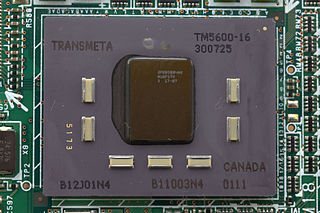
\includegraphics[width=0.5\textwidth]{imgs/Transmeta_TM5600}
  \caption{A Transmeta CPU from a Fujitsu laptop}
\end{figure}

